\chapter[SCP-001 一份记录]{
	Kate McTiriss - A Record \\
	SCP-001 一份记录
}

\label{chap:SCP-001.a.record}

\begin{figure}[H]
	\centering
	\captionsetup{justification=centering}
	
\includegraphics[width=\linewidth]{images/SCP.001.a.record.png}
	\caption*{下列收容措施由站点主管全体执行委员会(Site Directors' Executive Committee of the Whole)\\ 和O5议会全体一致通过}
\end{figure}

\bb{项目编号:}SCP-001

\bb{项目等级:}Thaumiel\ii{(主观评价)}

\bb{特殊收容措施:}依照站点主管全体执行委员会\footnote{\ii{SDECotW}。}于20██年5月3日一致作出的主观意见, SCP-001的数据库访问位置将被禁止编辑,仅可由O5议会成员所有的7份私人密钥修改。SDECotW的多数主观意见认为那之前被分类为SCP-001的物体不应再被给予SCP分类,并应当转存到Site-19的标准高价值收容锁柜中。

SDECotW全体一致认为任何情况下都不应在基金会数据库的SCP-001页面上做出客观宣言或陈述, 且只应有对过往基金会管理层意见的可证实真实记录。

根据O5议会在20██5月3日作出的多数意见,若Thaumiel实体,Mary Nakayama博士,或任何宣称是此人的实体与SCP基金会进行了接触,应该将其引导至O5议会以求进行谈判或合作。O5议会的多数意见认为当前不应该去尝试消灭Thaumiel实体、或是去尝试找到SCP-001数据库位置的薄弱点。

\bb{描述:}SDECotW和O5议会于20██5月3日全体一致认为,任何在特定SCP基金会数据库页面\bb{$\boldsymbol\odot$\slash Procedures\slash 001\slash SCP-001.fmtl}上做出的事实性称述都会变为客观事实。该意见认为对这一页面做出的任何修改都会造成范围极其广阔、且很可能是无限范围的阿尔法室(“终极关注”)型现实修改情形;SDECotW和O5议会认为不应再对此效应进行更多测试,理由是这种测试有极高可能引发潜在的XK/CK/LK/VK/ZK/תK级情景。

SDECotW全体一致认为其它在基金会数据库\bb{$\boldsymbol\odot$\slash Procedures\slash 001\slash}部分下的页面没有异常效应,使SCP-001效应被发现、并有可能创造出了Thaumiel实体的SCP-001数据过往版本应作为子页面储存在此目录下以供参考。

SDECotW全体一致认为必须对基金会数据库的所有空白位置进行检查,确认是否有更多的阿尔法室型现实修改异常;此外任何时候最多只能开放1000个经过彻底检查的数据库位供员工编辑新的特殊收容措施。

% =====

\clearpage
\tred{$\triangleright\ \odot$\slash Procedures\slash 001\slash Past\slash Feb_18,_20██_1.ftml}

\begin{scpbox}
\bb{基金会数据库修改记录:} \\
创建新SCP文件。在2███位置进行创建尝试,但项目的效应可能会让它自动移动到-001去。已让管理员解锁空白的001位置(为什么要空着?我想是图个方便)以防万一。 \\
- \ii{mnakayama},20██年2月18日11:34 AM
\end{scpbox}

\begin{figure}[H]
	\centering
	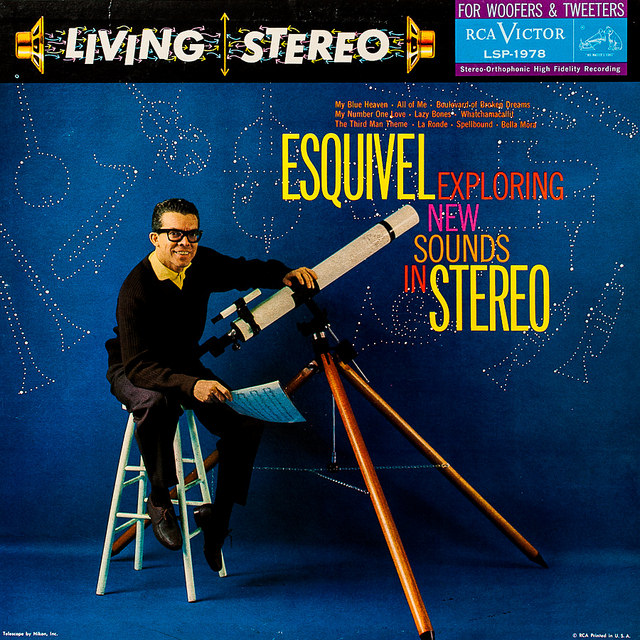
\includegraphics[width=0.5\linewidth]{images/SCP.001.a.record.2.jpg}
	\caption*{SCP-001的封面。唱片封面和无异常的再版封面相同。}
\end{figure}

\bb{项目编号:}SCP-001

\bb{项目等级:}Safe

\bb{特殊收容措施:}SCP-001将被收容于Site-91a的标准低价值收容锁柜中。对SCP-001效应的更多研究将由Site-91a首席数字命理学家Mary Nakayama博士负责。

描述:SCP-001是一张乙烯基唱片,内容为Esquivel发行于1958年的唱片《探索立体新声》(RCA)。该唱片会对将其纳入其中的数据化数字列表产生异常影响。若将该唱片列入数据保存的文本中,它将总是会被第一个列出,即便有意将其调至其他位置也是如此。\footnote{这一效应会扩散到一切形式的数据存储中。迄今受影响设备包括使用级电脑、移动电话、图表计算器。机械式存储设备,如书写或以物理形式表现地列表不会受到其异常效应影响。\label{footnote 2}}

SCP-001在1958年于发行前作为赠审阅副本送给了《公告牌》杂志。其效应一直未被发现,直至20██年十二月,《公告牌》杂志实习生M. S██████在将杂志总部过往审阅唱片的手工文件更新到数据库上时才发觉到其异常并向其上级进行了报告。\footnote{最初这起事件中可能的电子犯罪嫌疑引起了FBI注意。FBI电子犯罪部门内潜伏的UIU特工在发现该物品后将其给了基金会保管。\label{footnote 3}}

正在定位将SCP-001送到《公告牌》杂志的RCA员工。主流收容理论当前认为SCP-001是被用于试尝操控《公告牌》杂志的唱片排行榜,但由于当时该杂志还在使用人工打字,这一企图未能实现。

% =====

\clearpage
\tred{$\triangleright\ \odot$\slash Procedures\slash 001\slash Past\slash Feb_18,_20██_2.ftml}

\begin{scpbox}
\bb{基金会数据库修改记录:} \\
很好,真的自己移动过来了。奇怪。有趣。准备继续深入(可能有些隐藏的?)此外,修复了一个打字错误,感谢Dr Amoralles。 \\
- \ii{mnakayama},20██年2月18日11:41 AM
\end{scpbox}

\begin{figure}[H]
	\centering
	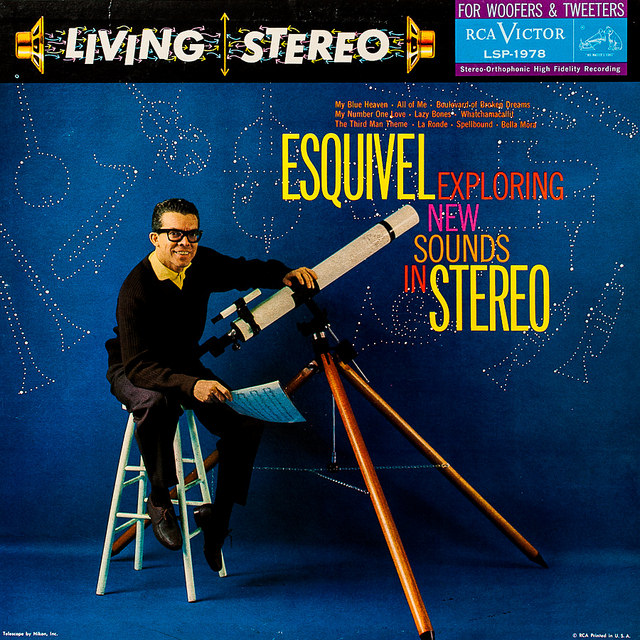
\includegraphics[width=0.5\linewidth]{images/SCP.001.a.record.2.jpg}
	\caption*{SCP-001的封面。唱片封面和无异常的再版封面相同。}
\end{figure}

\bb{项目编号:}SCP-001

\bb{项目等级:}Safe

\bb{特殊收容措施:}SCP-001将被收容于Site-91a的标准低价值收容锁柜中。对SCP-001效应的更多研究将由Site-91a首席数字命理学家Mary Nakayama博士负责。

\bb{描述:}SCP-001是一张乙烯基唱片,内容为Esquivel发行于1958年的唱片《探索立体新声》 (RCA)。该唱片会对将其纳入其中的数据化数字列表产生异常影响。若将该唱片列入数据保存的文本中,它将总是会被第一个列出,即便有意将其调至其他位置也是如此。

SCP-001在1958年于发行前作为审阅副本送给了《公告牌》杂志。其效应一直未被发现,直至20██年十二月,《公告牌》杂志实习生M. S██████在将杂志总部关于过往审阅唱片的手工打印文件更新到数据库上时才发觉到其异常并向其上级进行了报告。\footref{footnote 2}

正在定位将SCP-001送到《公告牌》杂志的RCA员工。主流收容理论当前认为SCP-001是被用于\red{\dd{试尝}}\green{尝试}操控《公告牌》杂志的唱片排行榜,但由于当时该杂志还在使用人工打字,这一企图未能实现。\footref{footnote 3}

% =====

\clearpage
\tred{$\triangleright\ \odot$\slash Procedures\slash 001\slash Past\slash Apr_1,_20██_1.ftml}

\begin{scpbox}
\bb{基金会数据库修改记录:} \\
对收容措施进行为期一天的重要修正 ;) \\
- \ii{mnakayama},20██4月1日9:41 AM
\end{scpbox}

\begin{figure}[H]
	\centering
	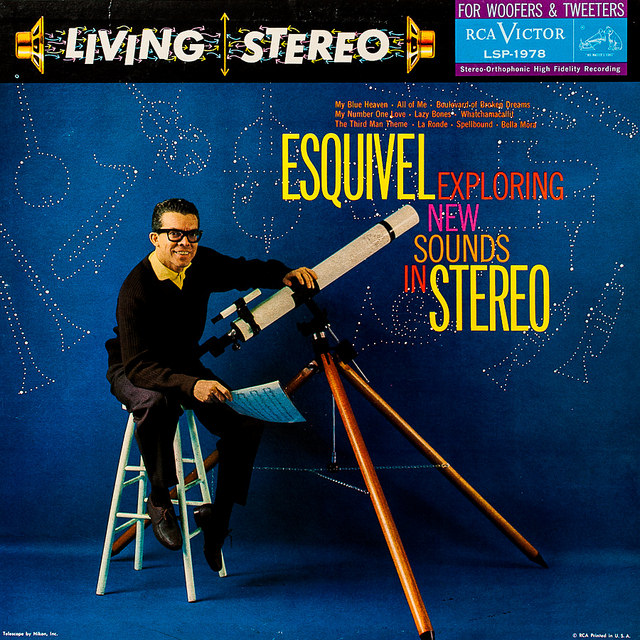
\includegraphics[width=0.5\linewidth]{images/SCP.001.a.record.2.jpg}
	\caption*{SCP-001的封面。唱片封面和无异常的再版封面相同。}
\end{figure}

\bb{项目编号:}SCP-001

\bb{项目等级:}Safe

\bb{特殊收容措施:}SCP-001将被收容于Site-91a的标准低价值收容锁柜中。对SCP-001效应的更多研究将由Site-91a首席数字命理学家Mary Nakayama博士负责。\green{所有Site-91a的2级研究员应当在20██年四月1日于Nakayama博士午餐时间向其支付5美元。}

\bb{描述:}SCP-001是一张乙烯基唱片,内容为Esquivel发行于1958年的唱片《探索立体新声》 (RCA)。该唱片会对将其纳入其中的数据化数字列表产生异常影响。若将该唱片列入数据保存的文本中,它将总是会被第一个列出,即便有意将其调至其他位置也是如此。

SCP-001在1958年于发行前作为审阅副本送给了《公告牌》杂志。其效应一直未被发现,直至20██年十二月,《公告牌》杂志实习生M. S██████在将杂志总部关于过往审阅唱片的手工打印文件更新到数据库上时才发觉到其异常并向其上级进行了报告。\footref{footnote 2}

正在定位将SCP-001送到《公告牌》杂志的RCA员工。主流收容理论当前认为SCP-001是被用于尝试操控《公告牌》杂志的唱片排行榜,但由于当时该杂志还在使用人工打字,这一企图未能实现。\footref{footnote 3}

% =====

\clearpage
\tred{$\triangleright\ \odot$\slash Procedures\slash 001\slash Past\slash Apr_1,_20██_2.ftml}

\begin{scpbox}
\bb{基金会数据库修改记录:} \\
这TM这TM这TM是·他·妈·的怎么回事。 \\
- \ii{mnakayama},20██年4月1日12:54 PM
\end{scpbox}

\begin{figure}[H]
	\centering
	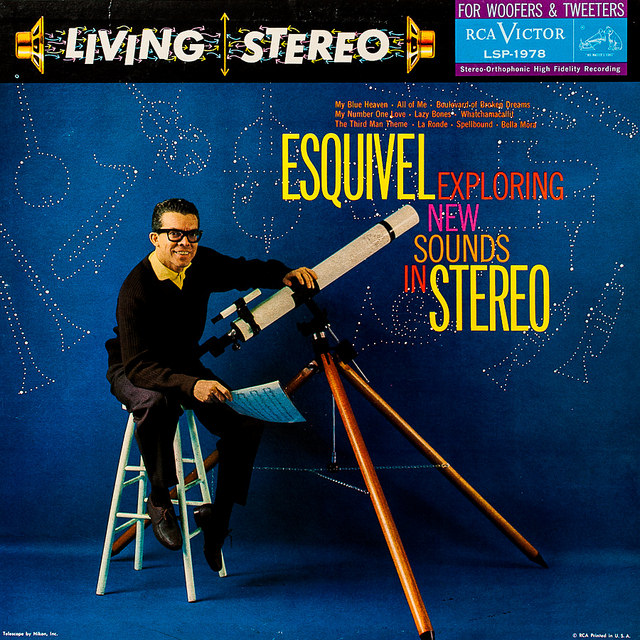
\includegraphics[width=0.5\linewidth]{images/SCP.001.a.record.2.jpg}
	\caption*{SCP-001的封面。唱片封面和无异常的再版封面相同。}
\end{figure}

\bb{项目编号:}SCP-001

\bb{项目等级:}Safe

\bb{特殊收容措施:}SCP-001将被收容于Site-91a的标准低价值收容锁柜中。对SCP-001效应的更多研究将由Site-91a首席数字命理学家Mary Nakayama博士负责。\red{\dd{所有Site-91a的2级研究员应当在20██年四月1日于Nakayama博士午餐时间向其支付5美元。}}

\bb{描述:}SCP-001是一张乙烯基唱片,内容为Esquivel发行于1958年的唱片《探索立体新声》 (RCA)。该唱片会对将其纳入其中的数据化数字列表产生异常影响。若将该唱片列入数据保存的文本中,它将总是会被第一个列出,即便有意将其调至其他位置也是如此。

SCP-001在1958年于发行前作为审阅副本送给了《公告牌》杂志。其效应一直未被发现,直至20██年十二月,《公告牌》杂志实习生M. S██████在将杂志总部关于过往审阅唱片的手工打印文件更新到数据库上时才发觉到其异常并向其上级进行了报告。\footref{footnote 2}

正在定位将SCP-001送到《公告牌》杂志的RCA员工。主流收容理论当前认为SCP-001是被用于尝试操控《公告牌》杂志的唱片排行榜,但由于当时该杂志还在使用人工打字,这一企图未能实现。\footref{footnote 3}

% =====

\clearpage
\tred{$\triangleright\ \odot$\slash Procedures\slash 001\slash Past\slash Apr_1,_20██_3.ftml}

\begin{scpbox}
\bb{基金会数据库修改记录:} \\
一些小测试。 \\
- \ii{mnakayama},20██4月1日9:09 PM。
\end{scpbox}

\begin{figure}[H]
	\centering
	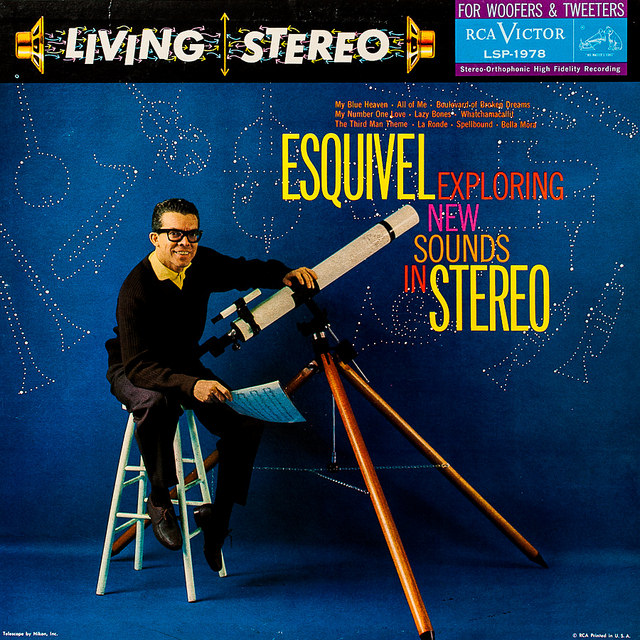
\includegraphics[width=0.5\linewidth]{images/SCP.001.a.record.2.jpg}
	\caption*{SCP-001的封面。唱片封面和无异常的再版封面相同。}
\end{figure}

\bb{项目编号:}SCP-001

\bb{项目等级:}Safe

\bb{特殊收容措施:}SCP-001将被收容于Site-91a的标准低价值收容锁柜中。对SCP-001效应的更多研究将由Site-91a首席数字命理学家Mary Nakayama博士负责。\green{Nakayama博士书桌上的名牌被染成绿色以便于识别。}

\bb{描述:}SCP-001是一张乙烯基唱片,内容为Esquivel发行于1958年的唱片《探索立体新声》 (RCA)。该唱片会对将其纳入其中的数据化数字列表产生异常影响。若将该唱片列入数据保存的文本中,它将总是会被第一个列出,即便有意将其调至其他位置也是如此。

SCP-001在1958年于发行前作为审阅副本送给了《公告牌》杂志。其效应一直未被发现,直至20██年十二月,《公告牌》杂志实习生M. S██████在将杂志总部关于过往审阅唱片的手工打印文件更新到数据库上时才发觉到其异常并向其上级进行了报告。\footref{footnote 2}

正在定位将SCP-001送到《公告牌》杂志的RCA员工。主流收容理论当前认为SCP-001是被用于尝试操控《公告牌》杂志的唱片排行榜,但由于当时该杂志还在使用人工打字,这一企图未能实现。\footref{footnote 3}

% =====

\clearpage
\tred{$\triangleright\ \odot$\slash Procedures\slash 001\slash Past\slash Apr_2,_20██_1.ftml}

\begin{scpbox}
\bb{基金会数据库修改记录:} \\
给自己请了个假。 \\
- \ii{mnakayama},20██4月1日9:09 PM。
\end{scpbox}

\begin{figure}[H]
	\centering
	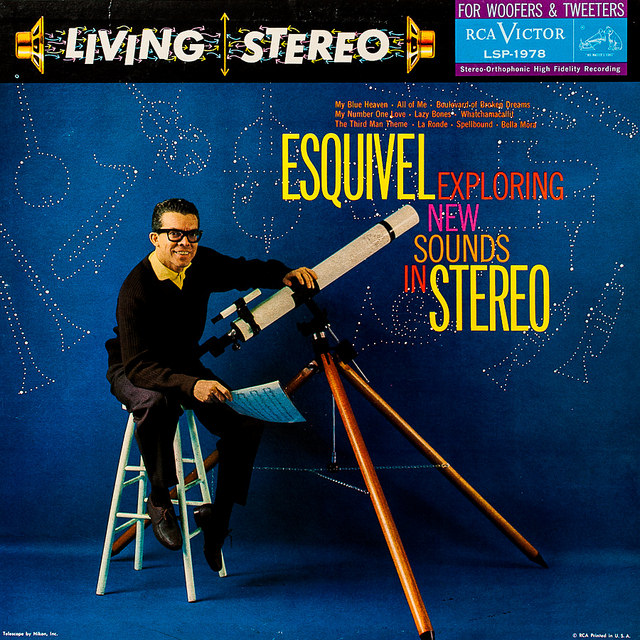
\includegraphics[width=0.5\linewidth]{images/SCP.001.a.record.2.jpg}
	\caption*{SCP-001的封面。唱片封面和无异常的再版封面相同。}
\end{figure}

\bb{项目编号:}SCP-001

\bb{项目等级:}Safe

\bb{特殊收容措施:}SCP-001将被收容于Site-91a的标准低价值收容锁柜中。对SCP-001效应的更多研究将由Site-91a首席数字命理学家Mary Nakayama博士负责。\red{\dd{Nakayama博士书桌上的名牌被染成绿色以便于识别。}}\green{通知所有人员Nakayama博士在20██4月9日前可能暂时不能工作,她已由站点主管Green批准在这期间休假。}

\bb{描述:}SCP-001是一张乙烯基唱片,内容为Esquivel发行于1958年的唱片《探索立体新声》 (RCA)。该唱片会对将其纳入其中的数据化数字列表产生异常影响。若将该唱片列入数据保存的文本中,它将总是会被第一个列出,即便有意将其调至其他位置也是如此。

SCP-001在1958年于发行前作为审阅副本送给了《公告牌》杂志。其效应一直未被发现,直至20██年十二月,《公告牌》杂志实习生M. S██████在将杂志总部关于过往审阅唱片的手工打印文件更新到数据库上时才发觉到其异常并向其上级进行了报告。\footref{footnote 2}

正在定位将SCP-001送到《公告牌》杂志的RCA员工。主流收容理论当前认为SCP-001是被用于尝试操控《公告牌》杂志的唱片排行榜,但由于当时该杂志还在使用人工打字,这一企图未能实现。\footref{footnote 3}

% =====

\clearpage
\tred{$\triangleright\ \odot$\slash Procedures\slash 001\slash Past\slash Apr_9,_20██_1.ftml}

\begin{scpbox}
\bb{基金会数据库修改记录:} \\
记录一下将要发生的头衔变动… \\
- \ii{mnakayama},20██4月1日9:09 PM。
\end{scpbox}

\begin{figure}[H]
	\centering
	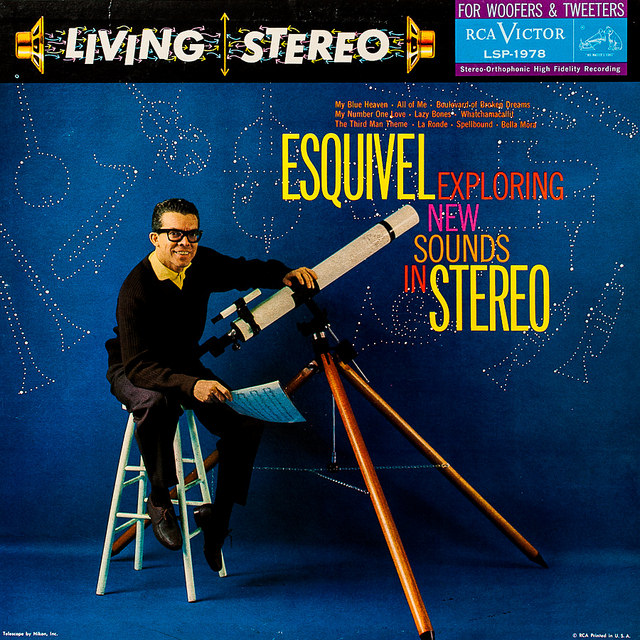
\includegraphics[width=0.5\linewidth]{images/SCP.001.a.record.2.jpg}
	\caption*{SCP-001的封面。唱片封面和无异常的再版封面相同。}
\end{figure}

\bb{项目编号:}SCP-001

\bb{项目等级:}Safe

\bb{特殊收容措施:}SCP-001将被收容于Site-91a的标准低价值收容锁柜中。对SCP-001效应的更多研究将由\red{\dd{Site-91a首席数字命理学家}}Mary Nakayama博士负责。\red{\dd{通知所有人员Nakayama博士在20██4月9日前可能暂时不能工作,她已由站点主管Green批准在这期间休假。}}\green{Nakayama博士,在4月9日以前的Site-91a首席数字命理学家,将在4月9日晚晋升为站点副主管协助Green博士工作。她将独立负责SCP-001项目。}

\bb{描述:}SCP-001是一张乙烯基唱片,内容为Esquivel发行于1958年的唱片《探索立体新声》 (RCA)。该唱片会对将其纳入其中的数据化数字列表产生异常影响。若将该唱片列入数据保存的文本中,它将总是会被第一个列出,即便有意将其调至其他位置也是如此。

SCP-001在1958年于发行前作为审阅副本送给了《公告牌》杂志。其效应一直未被发现,直至20██年十二月,《公告牌》杂志实习生M. S██████在将杂志总部关于过往审阅唱片的手工打印文件更新到数据库上时才发觉到其异常并向其上级进行了报告。\footref{footnote 2}

正在定位将SCP-001送到《公告牌》杂志的RCA员工。主流收容理论当前认为SCP-001是被用于尝试操控《公告牌》杂志的唱片排行榜,但由于当时该杂志还在使用人工打字,这一企图未能实现。\footref{footnote 3}

% =====

\clearpage
\tred{$\triangleright\ \odot$\slash Procedures\slash 001\slash Past\slash May_3,_20██_1.ftml}

\begin{scpbox}
\bb{基金会数据库修改记录:} \\
很好。一切如我所想。我已经准备了好几个星期;现在是时候了。我已经把这个页面对所有人锁定,除了我自己和O5们。我想我是在做一件正确的事。这是我的真实想法。为我祈祷吧。 \\
- \ii{mnakayama},20██5月3日4:11 AM。
\end{scpbox}

\bb{项目编号:}SCP-001

\red{\dd{\bb{项目等级:}Safe}}

\red{\dd{\bb{特殊收容措施:}SCP-001将被收容于Site-91a的标准低价值收容锁柜中。对SCP-001效应的更多研究将由Mary Nakayama博士负责。Nakayama博士,在4月9日以前的Site-91a首席数字命理学家,将在4月9日晚晋升为站点副主管协助Green博士工作。她将独立负责SCP-001项目。}}

\red{\dd{\bb{描述:}SCP-001是一张乙烯基唱片,内容为Esquivel发行于1958年的唱片《探索立体新声》 (RCA)。该唱片会对将其纳入其中的数据化数字列表产生异常影响。若将该唱片列入数据保存的文本中,它将总是会被第一个列出,即便有意将其调至其他位置也是如此。\footref{footnote 2}}}

\red{\dd{SCP-001在1958年于发行前作为赠审阅副本送给了《公告牌》杂志。其效应一直未被发现,直至20██年十二月,《公告牌》杂志实习生M. S██████在将杂志总部过往审阅唱片的手工文件更新到数据库上时才发觉到其异常并向其上级进行了报告。\footref{footnote 3}}}

\red{\dd{正在定位将SCP-001送到《公告牌》杂志的RCA员工。主流收容理论当前认为SCP-001是被用于尝试操控《公告牌》杂志的唱片排行榜,但由于当时该杂志还在使用人工打字,这一企图未能实现。}}

\green{Mary Nakayama,在本文档保存后立刻获得全知与全能,扬升到并成为神。她将超越一切时间,对这宇宙和现实具有完全的统治权。一切事物,一切事物之下的事物以及一切事物之上的事物,都将服从于她的命令。她将得到对在保持和利用这些能力的同时能维持自身意识清醒持续的一切必要心灵性质。}

\green{O5议会成员收到一份说明SCP-001性质的笔记。}

\green{她的家人将收到一份笔记,其中会表明她对他们的爱。}

\begin{scpbox}
Mary Nakayama在5月3日晚六点前从Site 91的宿舍中失踪。至今仍未被找到。
\end{scpbox}

% =====

\tred{$\triangleright$ 20██年5月3日早存入Mary Nakayama电脑内的文件}

\cl{
致O5议会,

在我十五岁时,我曾吃下过可以杀死我四次的药,给自己灌了一整瓶廉价伏特加,这是那个利用了我又把我抛下、任我心碎孤单的男人唯一留下的东西。

我坐在浴盆里任由热水炽烫我的身体。我闭上了眼睛。

当我睁开眼,我身上的水已经干了。一切安好。我躺在床上。在门边,一个闪烁的身影,发着光芒。盘旋着。它用一个只在我心中回响的声音向我开口说话。它说我有更伟大的事要做。

我再也没有看见过它。但我仍在继续前行。我相信那是上帝降临拯救了我。而,加入基金会后,我还怎么可能不相信呢?还有别的理由能解释为何我们仍存在于此、仍奇迹般地、绝望地、尖叫地活着的事实么?还有别的理由能解释我们世界的根基,我们的一切,竟能经受住这些我们每日面对的异物么?我们被保护着。我每夜向它祈祷指引。我再也未能听到那声音。

我曾触到上帝,那是改变我一生命运的时刻。

但当我在一篇文档上按下“保存”就把自己桌上的名牌变色时,我意识到了什么。万事万物的根基已向我开启。我本可抛下这力量,向你们报告,或者隐瞒它,但…

若这就是拯救我们的关键呢?如果它就是拯救我们所有人的关键,如果就是它在每一天从那些撕碎我们世界脆弱稳定的深渊噩梦手中保护着我们呢? 如果在一个文本里按下“保存”真的就是上帝的诞生呢?

若它不是,那就让我来尝试。若它就是,那就让我来监控它。我会试着将一切纠正。这可能会花些时间。

祝我好运。

- \ii{MN}
}

